\documentclass{exercise}

\institute{Applied and Computational Mathematics}
\title{Hausaufgabenübung 3}
\author{Joshua Feld, 406718}
\course{Mathematische Grundlagen IV}
\professor{Torrilhon \& Berkels}
\semester{Sommersemester 2022}
\program{CES (Bachelor)}

\begin{document}
    \maketitle


    \section*{Aufgabe 1}

    \begin{problem}
        Bestimmen Sie für die Funktion
        \[
            f\parentheses*{x} = 2\cos\parentheses*{x} + 2\sin\parentheses*{3x}
        \]
        mithilfe der acht Stützstellen \(x_k = \frac{2\pi k}{8}, k = 0, \ldots, 7\) die Koeffizienten \(c_l \in \C, l = 0, \ldots, 7\) des komplexen trigonometrischen Interpolationspolynoms:
        \begin{align*}
            T_8\parentheses*{f; x} &= \sum_{l = 0}^7 c_l e^{ilx}\\
            T_8\parentheses*{f; x_k} &= f\parentheses*{x_k}, \quad k = 0, \ldots, 7
        \end{align*}
        über die schnelle Fourier-Transformation, d.h. mit einem Algorithmus in \(\mathcal{O}\parentheses*{n\log n}\).
        Hierbei kann es hilfreich sein, die Teilprobleme in einem Binärbaum darzustellen.
    \end{problem}

    \subsection*{Lösung}
    \begin{center}
        \begin{tabular}{ccll}
            \toprule
            \(k\) & \(x_k\) & \(f\parentheses*{x_k}\) & \(= y_k\)\\
            \midrule
            \(0\) & \(0\) & \(2\sin\parentheses*{0} + 2\cos\parentheses*{0}\) & \(= 2\)\\
            \(1\) & \(\frac{\pi}{4}\) & \(2\sin\parentheses*{\frac{3\pi}{4}} + 2\cos\parentheses*{\frac{\pi}{4}} = 2 \cdot \frac{\sqrt{2}}{2} + 2 \cdot \frac{\sqrt{2}}{2}\) & \(= 2\sqrt{2}\)\\
            \(2\) & \(\frac{\pi}{2}\) & \(2\sin\parentheses*{\frac{3\pi}{2}} + 2\cos\parentheses*{\frac{\pi}{2}}\) & \(= -2\)\\
            \(3\) & \(\frac{3\pi}{4}\) & \(2\sin\parentheses*{\frac{9\pi}{4}} + 2\cos\parentheses*{\frac{3\pi}{4}} = 2 \cdot \frac{\sqrt{2}}{2} - 2 \cdot \frac{\sqrt{2}}{2}\) & \(= 0\)\\
            \(4\) & \(\pi\) & \(2\sin\parentheses*{3\pi} + 2\cos\parentheses*{\pi}\) & \(= -2\)\\
            \(5\) & \(\frac{5\pi}{4}\) & \(2\sin\parentheses*{\frac{15\pi}{4}} + 2\cos\parentheses*{\frac{5\pi}{4}} = -2 \cdot \frac{\sqrt{2}}{2} - 2 \cdot \frac{\sqrt{2}}{2}\) & \(= -2\sqrt{2}\)\\
            \(6\) & \(\frac{3\pi}{2}\) & \(2\sin\parentheses*{\frac{9\pi}{2}} + 2\cos\parentheses*{\frac{3\pi}{2}}\) & \(= 2\)\\
            \(7\) & \(\frac{7\pi}{4}\) & \(2\sin\parentheses*{\frac{21\pi}{4}} + 2\cos\parentheses*{\frac{7\pi}{4}} = -2 \cdot \frac{\sqrt{2}}{2} + 2 \cdot \frac{\sqrt{2}}{2}\) & \(= 0\)\\
            \bottomrule
        \end{tabular}
    \end{center}
    Das trigonometrische Interpolationspolynom ist gegeben durch
    \[
        T_n\parentheses*{x} = \sum_{j = 0}^{n - 1}d_j\parentheses*{f}e^{ijx}
    \]
    mit den Entwicklungskoeffizienten
    \[
        d_j\parentheses*{f} = \frac{1}{n}\sum_{l = 0}^{n - 1}y_l e^{-ijx_l}.
    \]
    Für gerades \(n\) gilt mit \(m = \frac{n}{2}\):
    \begin{align*}
        d_{2k} &= \frac{1}{2m}\sum_{j = 0}^{2m - 1}y_j e^{-2ikx_j}\\
        &= \frac{1}{m}\sum_{j = 0}^{m - 1}\frac{1}{2}\parentheses*{y_j + y_{j + m}}e^{-\frac{2\pi ikj}{m}}\\
        &= \frac{1}{m}\sum_{j = 0}^{m - 1}y_j^g e^{-ik\tilde{x}_j} = d_k^g\\
        d_{2k + 1} &= \frac{1}{m}\sum_{j = 0}^{m - 1}\underbrace{\frac{1}{2}\parentheses*{y_j - y_{j + m}}e^{-\frac{2\pi ij}{n}}}_{=: y_j^u}e^{-\frac{2\pi ikj}{m}}\\
        &= \frac{1}{m}\sum_{j = 0}^{m - 1}y_j^u e^{-ik\tilde{x}_j} = d_k^u.
    \end{align*}
    Die Koeffizienten \(d_k^g\) und \(d_k^u\) können nun als Fourierkoeffizienten von Interpolationspolynomen mit Stützstellen \(\tilde{x}_j = j\frac{2\pi}{m}\) aufgefasst werden mit den Funktionsauswertungen \(y_j^g\) bzw. \(y_j^u\).
    Ist nun \(m\) wieder gerade, so kann dieser Prozess wiederholt werden.
    Dies kann als Baumstruktur dargestellt werden.
    \begin{center}
        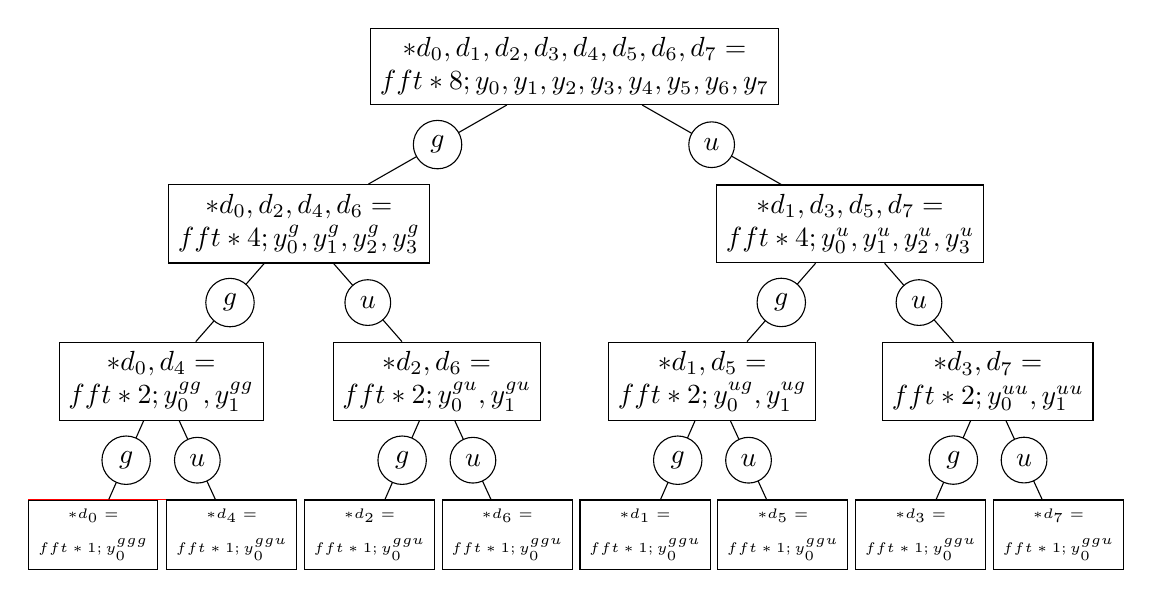
\begin{tikzpicture}
            \node[anchor=center,align=center,draw] (a) at (6.9375,5.5) {\(\brackets*{d_0, d_1, d_2, d_3, d_4, d_5, d_6, d_7} =\)\\\(fft\parentheses*{8; y_0, y_1, y_2, y_3, y_4, y_5, y_6, y_7}\)};
            \node[anchor=center,align=center,draw] (g) at (3.4375,3.5) {\(\brackets*{d_0, d_2, d_4, d_6} =\)\\\(fft\parentheses*{4; y_0^g, y_1^g, y_2^g, y_3^g}\)};
            \node[anchor=center,align=center,draw] (u) at (10.4375,3.5) {\(\brackets*{d_1, d_3, d_5, d_7} =\)\\\(fft\parentheses*{4; y_0^u, y_1^u, y_2^u, y_3^u}\)};
            \node[anchor=center,align=center,draw] (gg) at (1.6875,1.5) {\(\brackets*{d_0, d_4} =\)\\\(fft\parentheses*{2; y_0^{gg}, y_1^{gg}}\)};
            \node[anchor=center,align=center,draw] (gu) at (5.1875,1.5) {\(\brackets*{d_2, d_6} =\)\\\(fft\parentheses*{2; y_0^{gu}, y_1^{gu}}\)};
            \node[anchor=center,align=center,draw] (ug) at (8.6875,1.5) {\(\brackets*{d_1, d_5} =\)\\\(fft\parentheses*{2; y_0^{ug}, y_1^{ug}}\)};
            \node[anchor=center,align=center,draw] (uu) at (12.1875,1.5) {\(\brackets*{d_3, d_7} =\)\\\(fft\parentheses*{2; y_0^{uu}, y_1^{uu}}\)};
            \node[anchor=north west,align=center,draw] (ggg) at (0,0) {\tiny\(\brackets*{d_0} =\)\\\tiny\(fft\parentheses*{1; y_0^{ggg}}\)};
            \draw[red] (0,0) -- (3.375,0);
            \node[anchor=north west,align=center,draw] (ggu) at (1.75,0) {\tiny\(\brackets*{d_4} =\)\\\tiny\(fft\parentheses*{1; y_0^{ggu}}\)};
            \node[anchor=north west,align=center,draw] (gug) at (3.5,0) {\tiny\(\brackets*{d_2} =\)\\\tiny\(fft\parentheses*{1; y_0^{ggu}}\)};
            \node[anchor=north west,align=center,draw] (guu) at (5.25,0) {\tiny\(\brackets*{d_6} =\)\\\tiny\(fft\parentheses*{1; y_0^{ggu}}\)};
            \node[anchor=north west,align=center,draw] (ugg) at (7,0) {\tiny\(\brackets*{d_1} =\)\\\tiny\(fft\parentheses*{1; y_0^{ggu}}\)};
            \node[anchor=north west,align=center,draw] (ugu) at (8.75,0) {\tiny\(\brackets*{d_5} =\)\\\tiny\(fft\parentheses*{1; y_0^{ggu}}\)};
            \node[anchor=north west,align=center,draw] (uug) at (10.5,0) {\tiny\(\brackets*{d_3} =\)\\\tiny\(fft\parentheses*{1; y_0^{ggu}}\)};
            \node[anchor=north west,align=center,draw] (uuu) at (12.25,0) {\tiny\(\brackets*{d_7} =\)\\\tiny\(fft\parentheses*{1; y_0^{ggu}}\)};
            \draw (a) -- (g) node[draw,circle,fill=white,midway] {\(g\)};
            \draw (a) -- (u) node[draw,circle,fill=white,midway] {\(u\)};
            \draw (g) -- (gg) node[draw,circle,fill=white,midway] {\(g\)};
            \draw (g) -- (gu) node[draw,circle,fill=white,midway] {\(u\)};
            \draw (u) -- (ug) node[draw,circle,fill=white,midway] {\(g\)};
            \draw (u) -- (uu) node[draw,circle,fill=white,midway] {\(u\)};
            \draw (gg) -- (ggg) node[draw,circle,fill=white,midway] {\(g\)};
            \draw (gg) -- (ggu) node[draw,circle,fill=white,midway] {\(u\)};
            \draw (gu) -- (gug) node[draw,circle,fill=white,midway] {\(g\)};
            \draw (gu) -- (guu) node[draw,circle,fill=white,midway] {\(u\)};
            \draw (ug) -- (ugg) node[draw,circle,fill=white,midway] {\(g\)};
            \draw (ug) -- (ugu) node[draw,circle,fill=white,midway] {\(u\)};
            \draw (uu) -- (uug) node[draw,circle,fill=white,midway] {\(g\)};
            \draw (uu) -- (uuu) node[draw,circle,fill=white,midway] {\(u\)};
        \end{tikzpicture}
    \end{center}
    Damit ergibt sich
    \begin{align*}
        y_0^g &= \frac{1}{2}\parentheses*{y_0 + y_4} = 0, & y_0^u &= \frac{1}{2}\parentheses*{y_0 - y_4} = 2,\\
        y_1^g &= \frac{1}{2}\parentheses*{y_1 + y_5} = 0, & y_0^u &= \frac{1}{2}\parentheses*{y_1 - y_5}e^{-i\frac{\pi}{4}} = 2 - 2i,\\
        y_2^g &= \frac{1}{2}\parentheses*{y_2 + y_6} = 0, & y_0^u &= \frac{1}{2}\parentheses*{y_2 - y_6}e^{-i\frac{\pi}{2}} = 2i,\\
        y_3^g &= \frac{1}{2}\parentheses*{y_3 + y_7} = 0, & y_0^u &= \frac{1}{2}\parentheses*{y_3 - y_7}e^{-i\frac{3\pi}{4}} = 0.
    \end{align*}
    Damit gilt weiter
    \begin{align*}
        y_0^{gg} &= \frac{1}{2}\parentheses*{y_0^g + y_2^g} = 0, & y_0^{ug} &= \frac{1}{2}\parentheses*{y_0^u + y_2^u} = 1 + i,\\
        y_1^{gg} &= \frac{1}{2}\parentheses*{y_1^g + y_3^g} = 0, & y_0^{ug} &= \frac{1}{2}\parentheses*{y_1^u + y_3^u} = 1 - i,\\
        y_0^{gu} &= \frac{1}{2}\parentheses*{y_0^g - y_2^g} = 0, & y_0^{ug} &= \frac{1}{2}\parentheses*{y_0^u - y_2^u} = 1 - i,\\
        y_1^{gu} &= \frac{1}{2}\parentheses*{y_1^g - y_3^g}e^{-i\frac{\pi}{2}} = 0, & y_0^{ug} &= \frac{1}{2}\parentheses*{y_1^u - y_3^u}e^{-i\frac{\pi}{2}} = -1 - i.
    \end{align*}
    Letztlich
    \begin{align*}
        y_0^{ggg} &= \frac{1}{2}\parentheses*{y_0^{gg} + y_1^{gg}} = 0 = d_0^{ggg} = d_0, & y_0^{ugg} &= \frac{1}{2}\parentheses*{y_0^{ug} + y_1^{ug}} = 1 = d_0^{ugg} = d_1,\\
        y_0^{ggu} &= \frac{1}{2}\parentheses*{y_0^{gg} - y_1^{gg}}e^{-i\pi} = 0 = d_0^{ggu} = d_4, & y_0^{ugu} &= \frac{1}{2}\parentheses*{y_0^{ug} - y_1^{ug}} = i = d_0^{ugu} = d_5,\\
        y_0^{gug} &= \frac{1}{2}\parentheses*{y_0^{gu} + y_1^{gu}} = 0 = d_0^{gug} = d_2, & y_0^{uug} &= \frac{1}{2}\parentheses*{y_0^{uu} + y_1^{uu}} = -i = d_0^{uug} = d_3,\\
        y_0^{guu} &= \frac{1}{2}\parentheses*{y_0^{gu} - y_1^{gu}} = 0 = d_0^{guu} = d_6, & y_0^{uuu} &= \frac{1}{2}\parentheses*{y_0^{uu} - y_1^{uu}} = 1 = d_0^{uuu} = d_7.
    \end{align*}
\end{document}
